% Drawing 138/04-6 -- folder 138, batch 04, archive page 77 (PDF page 78).
% Transcription: la double pyramide de la p.~63, redessinée : $E^{+}$ en haut (avec, à côté, « $\rho_0 =$ » laissé en suspens), $E^{-}$ en bas, l'équateur $D_{20}$, $D_{01}$, $D_{12}$, les points $S_0$, $S_1$, $S_2$ et les flèches $\pi_0^{\pm}$, $\pi_1^{\pm}$, $\pi_2^{\pm}$.
% Kind: double pyramid (redrawn, pencil). Method 2 (schematic redraw from the facsimile). Status: partial.
% Notes: The double pyramid of p. 63 redrawn in pencil: E+ at the top with « rho_0 = » left hanging, E- at the bottom, the equator D_20, D_01, D_12 (the label near D_12 reads « D_02 D_12 », kept as D_12), S_0, S_1, S_2, the arrows pi^pm_i. Faint pencil: the back edges and the arrow heads are partly a reading.
% Coordinates: 1 unit = 1 mm = 1/100 of the crop width (bbox in page fractions: [0.08, 0.08, 0.44, 0.48]).
% Redrawn by Claude (claude-opus-5-5), issue #73, 2026-11-07; not checked by a human; not compiled (no TeX in the session).
% Rights: reproduces part of the work -- behind RENDER_TRANSCRIPTS, never published by itself.
\documentclass[tikz,border=3pt]{standalone}
\usepackage{amsmath,amssymb}
\usetikzlibrary{patterns,arrows.meta}
\tikzset{pencil/.style={black!45}, struck/.style={black!35}, mark/.style={circle,draw,inner sep=1.3pt}, pt/.style={circle,fill,inner sep=0.9pt}, opt/.style={circle,draw,fill=white,inner sep=1.1pt}}
\begin{document}
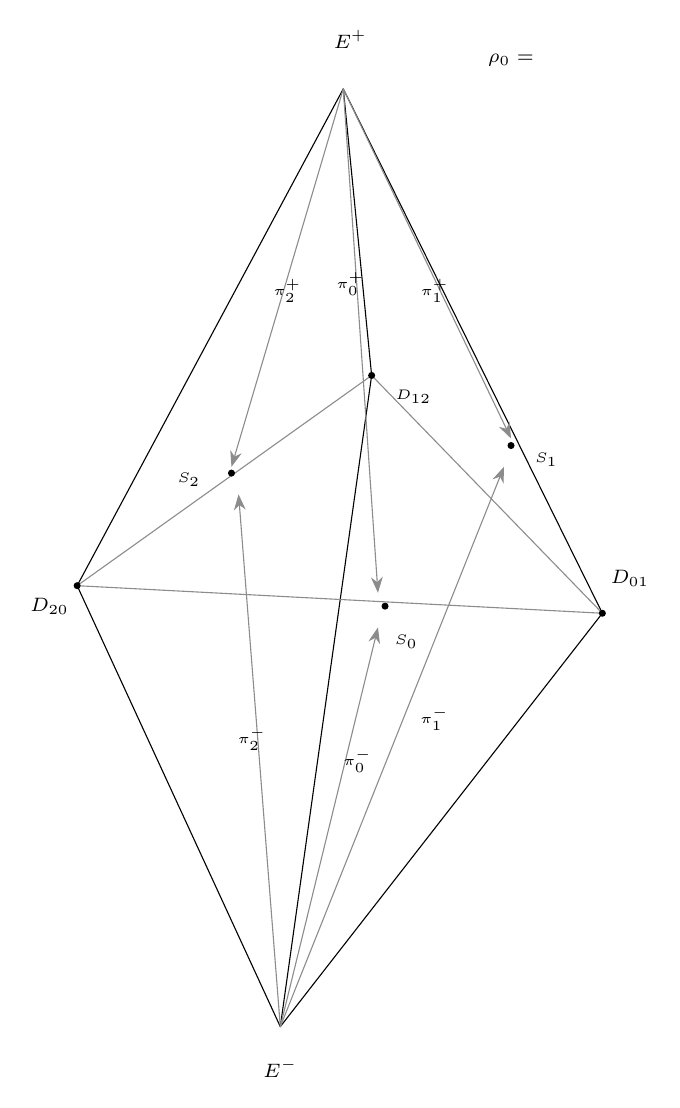
\begin{tikzpicture}[x=1mm,y=1mm,line cap=round,line join=round,font=\scriptsize]
\draw (64,-19.6) -- (30.2,-82.7);
\draw (64,-19.6) -- (96.9,-86.2);
\draw (56,-138.7) -- (30.2,-82.7);
\draw (56,-138.7) -- (96.9,-86.2);
\draw (64,-19.6) -- (67.6,-56);
\draw (56,-138.7) -- (67.6,-56);
\draw[pencil] (30.2,-82.7) -- (96.9,-86.2);
\draw[pencil] (30.2,-82.7) -- (67.6,-56);
\draw[pencil] (67.6,-56) -- (96.9,-86.2);
\draw[-{Stealth[length=2mm]},pencil] (64,-19.6) -- (49.8,-67.6);
\draw[-{Stealth[length=2mm]},pencil] (64,-19.6) -- (68.4,-83.6);
\draw[-{Stealth[length=2mm]},pencil] (64,-19.6) -- (85.3,-64);
\draw[-{Stealth[length=2mm]},pencil] (56,-138.7) -- (50.7,-71.1);
\draw[-{Stealth[length=2mm]},pencil] (56,-138.7) -- (68.4,-88);
\draw[-{Stealth[length=2mm]},pencil] (56,-138.7) -- (84.4,-67.6);
\node[pt] at (30.2,-82.7) {};
\node[pt] at (96.9,-86.2) {};
\node[pt] at (67.6,-56) {};
\node[pt] at (69.3,-85.3) {};
\node[pt] at (49.8,-68.4) {};
\node[pt] at (85.3,-64.9) {};
\node[inner sep=1pt] at (64.9,-13.3) {\scriptsize $E^{+}$};
\node[inner sep=1pt] at (85.3,-16) {\scriptsize $\rho_0=$};
\node[inner sep=1pt] at (56,-144) {\scriptsize $E^{-}$};
\node[inner sep=1pt] at (26.7,-85.3) {\scriptsize $D_{20}$};
\node[inner sep=1pt] at (100.4,-81.8) {\scriptsize $D_{01}$};
\node[inner sep=1pt] at (72.9,-58.7) {\tiny $D_{12}$};
\node[inner sep=1pt] at (72,-89.8) {\tiny $S_0$};
\node[inner sep=1pt] at (89.8,-66.7) {\tiny $S_1$};
\node[inner sep=1pt] at (44.4,-69.3) {\tiny $S_2$};
\node[inner sep=1pt] at (56.9,-45.3) {\tiny $\pi_2^{+}$};
\node[inner sep=1pt] at (64.9,-44.4) {\tiny $\pi_0^{+}$};
\node[inner sep=1pt] at (75.6,-45.3) {\tiny $\pi_1^{+}$};
\node[inner sep=1pt] at (52.4,-102.2) {\tiny $\pi_2^{-}$};
\node[inner sep=1pt] at (65.8,-104.9) {\tiny $\pi_0^{-}$};
\node[inner sep=1pt] at (75.6,-99.6) {\tiny $\pi_1^{-}$};
\end{tikzpicture}
\end{document}
